To be able to reliably use motors instead of sending just PWM data to motors there needs to be a node which translates linear and angular speeds to necessary PWM values. However as PWM vs speed relation is highly non-linear and depends on many factors such as ground friction it is not possible to just find suitable function for translating speed to PWM. The use of motor controller is therefore crucial. Its task is to control PWM values at the same time getting feedback from encoders. This data then can be used to adjust PWM values so that motor reaches the necessary speed and keeps it. In this project PID controller is used for motor control. Equation \ref{eq:pid_equation} shows general PID controller algorithm. In case of motor controller error e(t) is difference between desired angular speed and current angular speed which can be calculated with equation \ref{eq:pid_error}. $M$ describes ticks per revolution.

\begin{align}
\label{eq:pid_equation}
u(t) = K_p e(t) + K_i \int_{0}^{t} e(\tau) d\tau + K_d \frac{de(t)}{dt} 
\end{align}

\begin{align}
\label{eq:pid_error}
\omega (t) = \frac{2 \pi \Delta \text{encoder}}{\Delta t \cdot M}
\end{align}

With PID controller it is very important to find right parameters otherwise motion can be with oscillations, too slowly rising or could have other problems. 

For this project, we have the controller architecture shown in Figure \ref{fig:controller}.

\begin{figure}[h]    
\centering    
                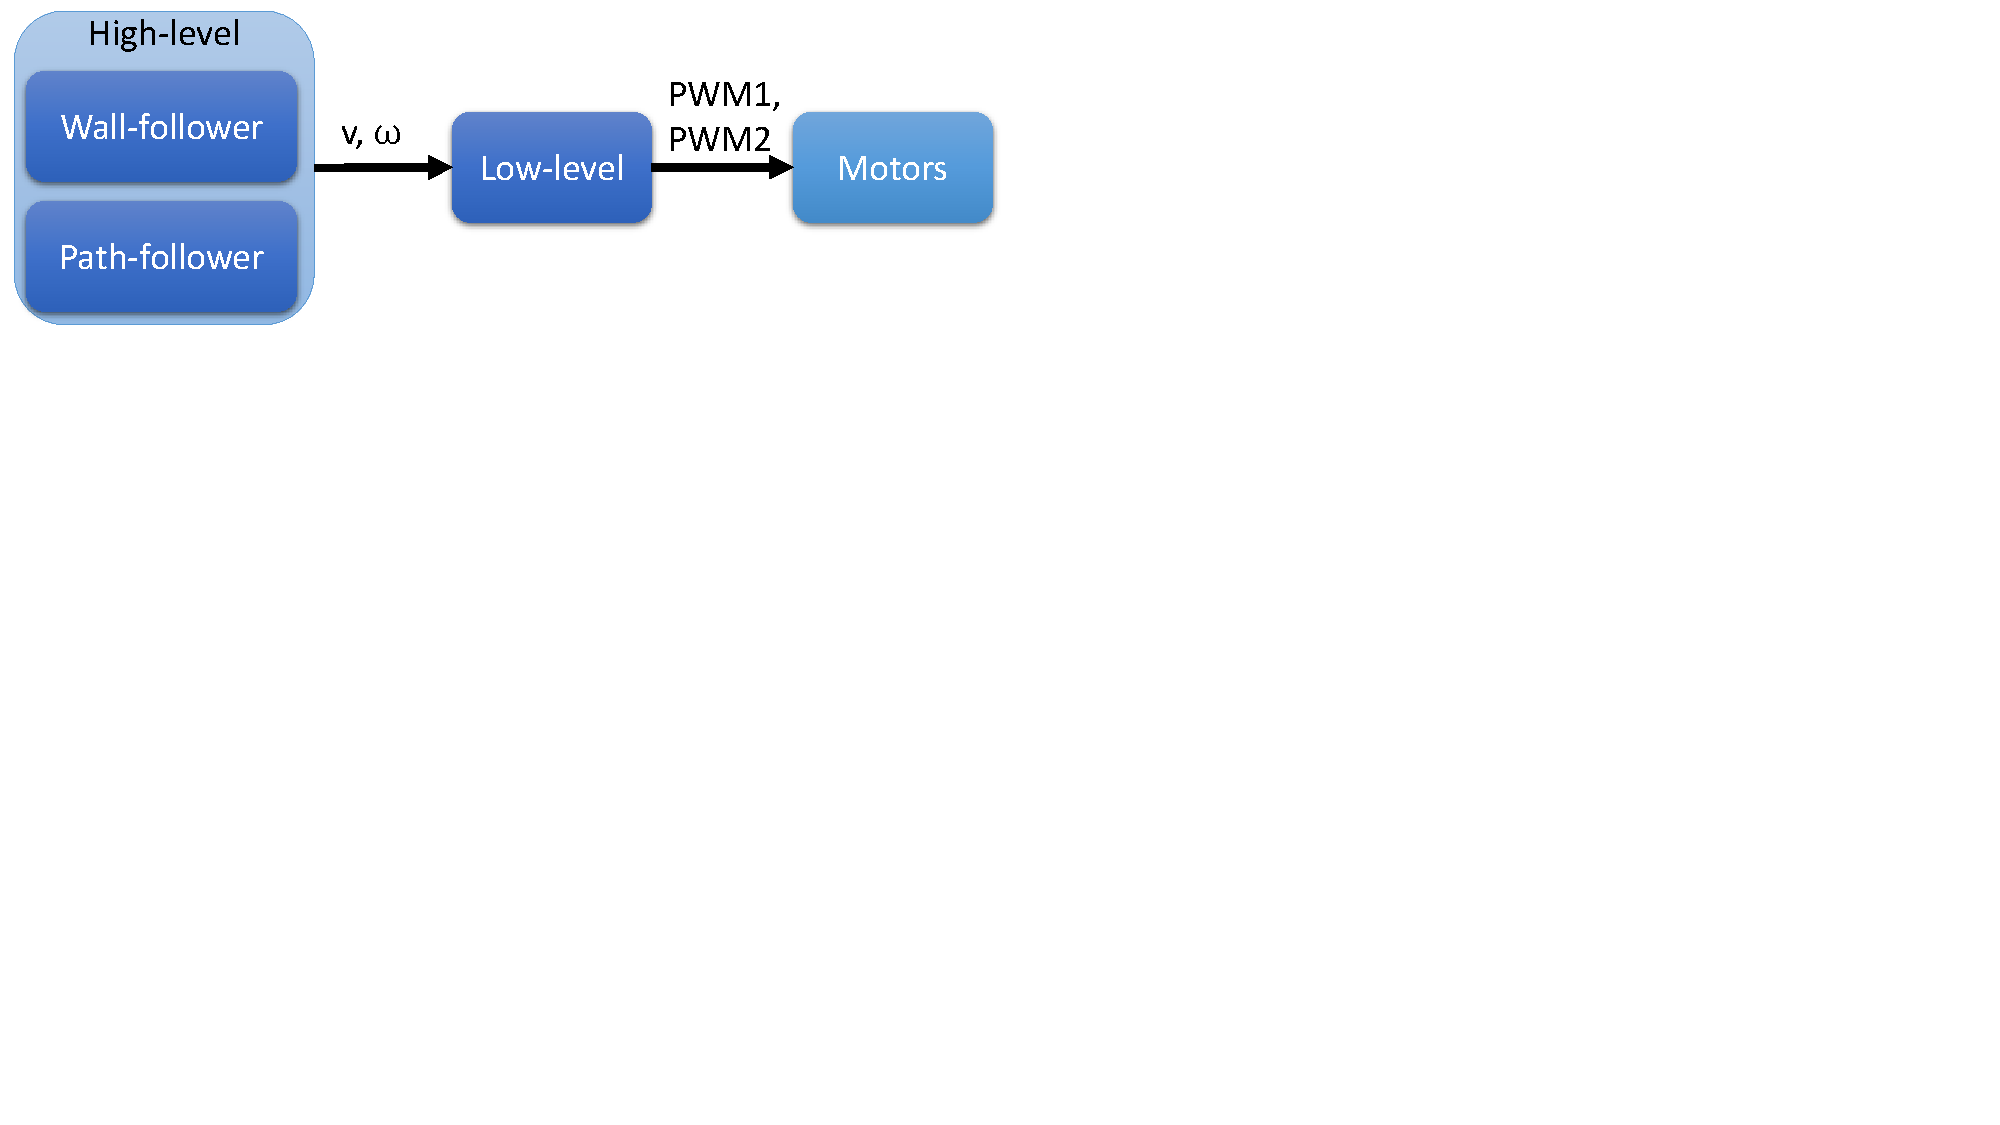
\includegraphics[trim = 0mm 130mm 170mm 0mm, clip, width=0.6\textwidth]{figures/controller.pdf}
                \caption{Controller architecture.}
                \label{fig:controller}
\end{figure}

In order to translate from $v$, $\omega$ to angular velocity for the wheel, we apply the following:
\begin{align}
\omega_l = \frac{(v - (B/2.0) \cdot \omega)}{R}\\
\omega_r = \frac{(v + (B/2.0) \cdot \omega)}{R}
\end{align}
, where $B$ is the distance between wheels, and $R$ is the wheel radio. 

\textbf{Remarks}\\
The main problem we found out is that the motors are \textbf{non-linear} in the low-power region: they require a minimum amount of PWM signal to start actually moving. We solved this by simply adding a constant value of 45 and 47 to the left and right motor PWM signal, respectively. This provided a much faster response from the PID controller. 